\documentclass{Phyport}
\usepackage{amsmath, amsthm, amssymb, amsfonts}
\usepackage{esint}
\usepackage{nicematrix}
\usepackage{extarrows}
\usepackage{graphicx}
\usepackage{enumitem}
\usepackage{multirow, booktabs}
\usepackage{caption}
\usepackage{float}
\usepackage[dvipsnames]{xcolor}
\usepackage[english]{babel}
\usepackage{bm}
\usepackage{cite}
\usepackage{multirow}
\usepackage{hyperref}
\hypersetup{
    colorlinks=true,
}
\usepackage{amsmath, amsthm, amssymb, amsfonts}
\usepackage{esint}
\usepackage{nicematrix}
\usepackage{extarrows}
\usepackage{graphicx}
\usepackage{enumitem}
\usepackage{multirow, booktabs}
\usepackage{caption}
\usepackage{float}
\usepackage[dvipsnames]{xcolor}
\usepackage{babel}
\usepackage{bm}
\usepackage{cite}

\renewcommand{\d}{\mathrm{d}}
\newcommand{\e}{\mathrm{e}}
\newcommand{\dv}[3][]{%
  \frac{\d^{#1} #2}{\d #3^{#1}}} %求n阶导数的Leibniz符号, 当n=1时第一个变量不填.
\newcommand{\pdv}[3][]{%
  \frac{\pa^{#1} #2}{\pa {#3}^{#1}}} %选用宏

\exname{光速测量} %实验名称
\extable{8} %实验桌号
\instructor{张利} %指导教师
\class{生医2402} %班级
\name{姚舜瑜} %姓名
\stuid{3240100532} %学号

\nyear{2025} %年
\nmonth{9} %月
\nday{23} %日
\nweekday{二} %星期几

\redate{} %如有实验补做,补做日期
\resitu{} %情况说明:

\begin{document}
\setcounter{page}{0}
\makecover


\section{预习报告(10分)}
\subsection{实验综述(5分)}
\subsubsection{实验原理}
本实验采用光调制法测量光速。基本原理如下:

假设我们让一个光源照射一个接收器,二者距离为$\Delta S$,我们就可以通过测量光信号到达接收器的时间差$\Delta t$,从而计算出光速$c=\frac{\Delta S}{\Delta t}$。
但由于光速极快,直接测量时间差$\Delta t$非常困难,因此我们采用相位法测量光速。我们使用一个周期性调制的光源发射光信号,其光强为$I=I_0 +\Delta I_0 \cos(2\pi \upsilon t)$。
将其转化为变化的电压信号$U=U_0 \cos(2\pi \upsilon t)$。我们通过测量光信号到达接收器时产生的电压信号与初始信号之间的相位差$\Delta \phi$,从而计算出时间差$\Delta t=\frac{\Delta \phi}{2\pi \upsilon }$,进而计算出光速$c=\frac{2\pi \upsilon  \Delta S}{\Delta \phi}$。

但由于此时,调制频率 $\upsilon $ 的值较大,光程 $\Delta S$ 很小的距离变化都可能引起相位差 $\Delta \phi$ 的急剧变化,用示波器难以精确测量。
因此,我们采用和差频法进行处理。将接收到的含有相位差 $\Delta \phi$ 的高频信号 $U_2 = A_2 \cos(2\pi \upsilon t - \Delta\phi)$ 与另一个频率为 $\upsilon ''$ 的高频信号 $U_3 = A_3 \cos(2\pi \upsilon ''t)$ 进行差频。
根据三角函数积化和差公式,混频后得到的信号为:
\begin{equation}
U_2 \cdot U_3 \propto \cos(2\pi(\upsilon +\upsilon '')t - \Delta\phi) + \cos(2\pi(\upsilon -\upsilon '')t - \Delta\phi)
\end{equation}

该信号包含一个和频分量和一个差频分量(忽略振幅)。
接着,使用一个滤波器滤除高频的和频信号,只保留低频的差频信号 $\upsilon ' = \upsilon  - \upsilon ''$。得到的最终信号为 $U' \propto \cos(2\pi \upsilon 't - \Delta\phi)$。
而处理后的低频信号 $U'$ 与原始高频信号 $U_2$ 具有完全相同的相位差 $\Delta\phi$。
这样,我们就可以通过精确测量容易观察的低频信号的相位差 $\Delta\phi$,来间接测量高频信号的相位差 $\Delta\phi$。

\begin{figure}[H]
    \centering
    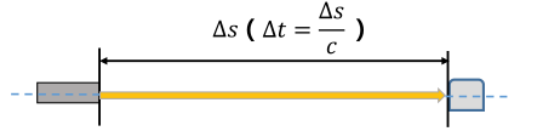
\includegraphics[width=0.6\textwidth]{理论原理图.png}
    \caption{相位法测量光速原理}
    \label{fig:相位法原理}
\end{figure}

在实验真实使用的光速测量仪器上,由于光源和接收器放在一起,光信号是经过反射镜反射后再到达接收器的,因此光程实际上是 $2\Delta S$。
那么高频信号的相位差为 $\Delta\phi = 2\pi \upsilon  \Delta t = 2\pi \upsilon  \frac{2\Delta S}{c}$,而低频信号的相位差为 $\Delta\phi = 2\pi \upsilon ' \Delta t'$,且两者相位差相等,
整理后即可得到最终用于计算光速的公式:

\begin{equation}
\label{eq:光速公式}
c = \frac{2(s_2 - s_1)\upsilon }{\Delta t' \upsilon '}
\end{equation}

其中,$s_2 - s_1$ 是光程差 $\Delta S$,$\upsilon $ 是原始高频频率, $\upsilon '$ 是差频频率,$\Delta t'$ 是在示波器上测得的低频信号时间差。

\begin{figure}[H]
    \centering
    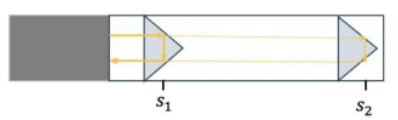
\includegraphics[width=0.4\textwidth]{真实仪器示意图.png}
    \caption{真实仪器示意图}
    \label{fig:真实仪器示意图}
\end{figure}

于是,根据上述理论原理,我们制造出了如下仪器:
\begin{figure}[H]
    \centering
    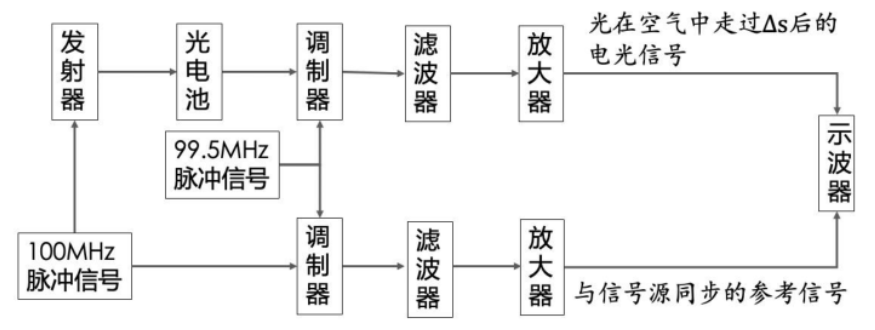
\includegraphics[width=0.8\textwidth]{仪器原理.png}
    \caption{仪器原理}
    \label{fig:仪器原理}
\end{figure}


\subsubsection{实验方法}
本实验主要器材包括:1、光速测量仪;2、示波器;


\textbf{Step 1.} 开启电源,调节光路,确保发射光能准确地反射回接收器中心,以获得最强的信号。

\textbf{Step 2.} 取第一个六等分点为$S_1$,利用示波器$Track$功能将光标1对齐测量信号幅度峰值。保持光标1位置不变。

\textbf{Step 3.} 移动反射镜到剩余的六个等分点$S_2$至$S_6$,每移动到一个点,利用示波器$Track$功能将光标2对齐测量信号幅度峰值,记录此时的时间差$\Delta t'$。

\textbf{Step 4.} 根据测得的六个时间差$\Delta t'$和对应的光程差$s_2 - s_1$,利用公式\eqref{eq:光速公式}计算出光速$c$的值。

\textbf{Step 5.} 略微改变$S_1$的位置,重复上述步骤,获取更多数据,计算平均值并估算误差。




\subsection{实验重点(3分)}
1. 理解相位法测量光速的基本原理和实验方法。

2. 学会通过“逐差法”或“累积法”减小测量误差。

\subsection{实验难点(2分)}
1. 光路调节:精确调节光路,确保发射光能准确地反射回接收器中心,以获得最强的信号。

2. 示波器使用:熟练掌握示波器的各项功能,特别是$Track$功能,以便准确测量信号的时间差。

3. 数据处理:合理处理测量数据,计算光速并估算误差。

\newpage


\section{原始数据(20分)}
\begin{figure}[H]
    \centering
    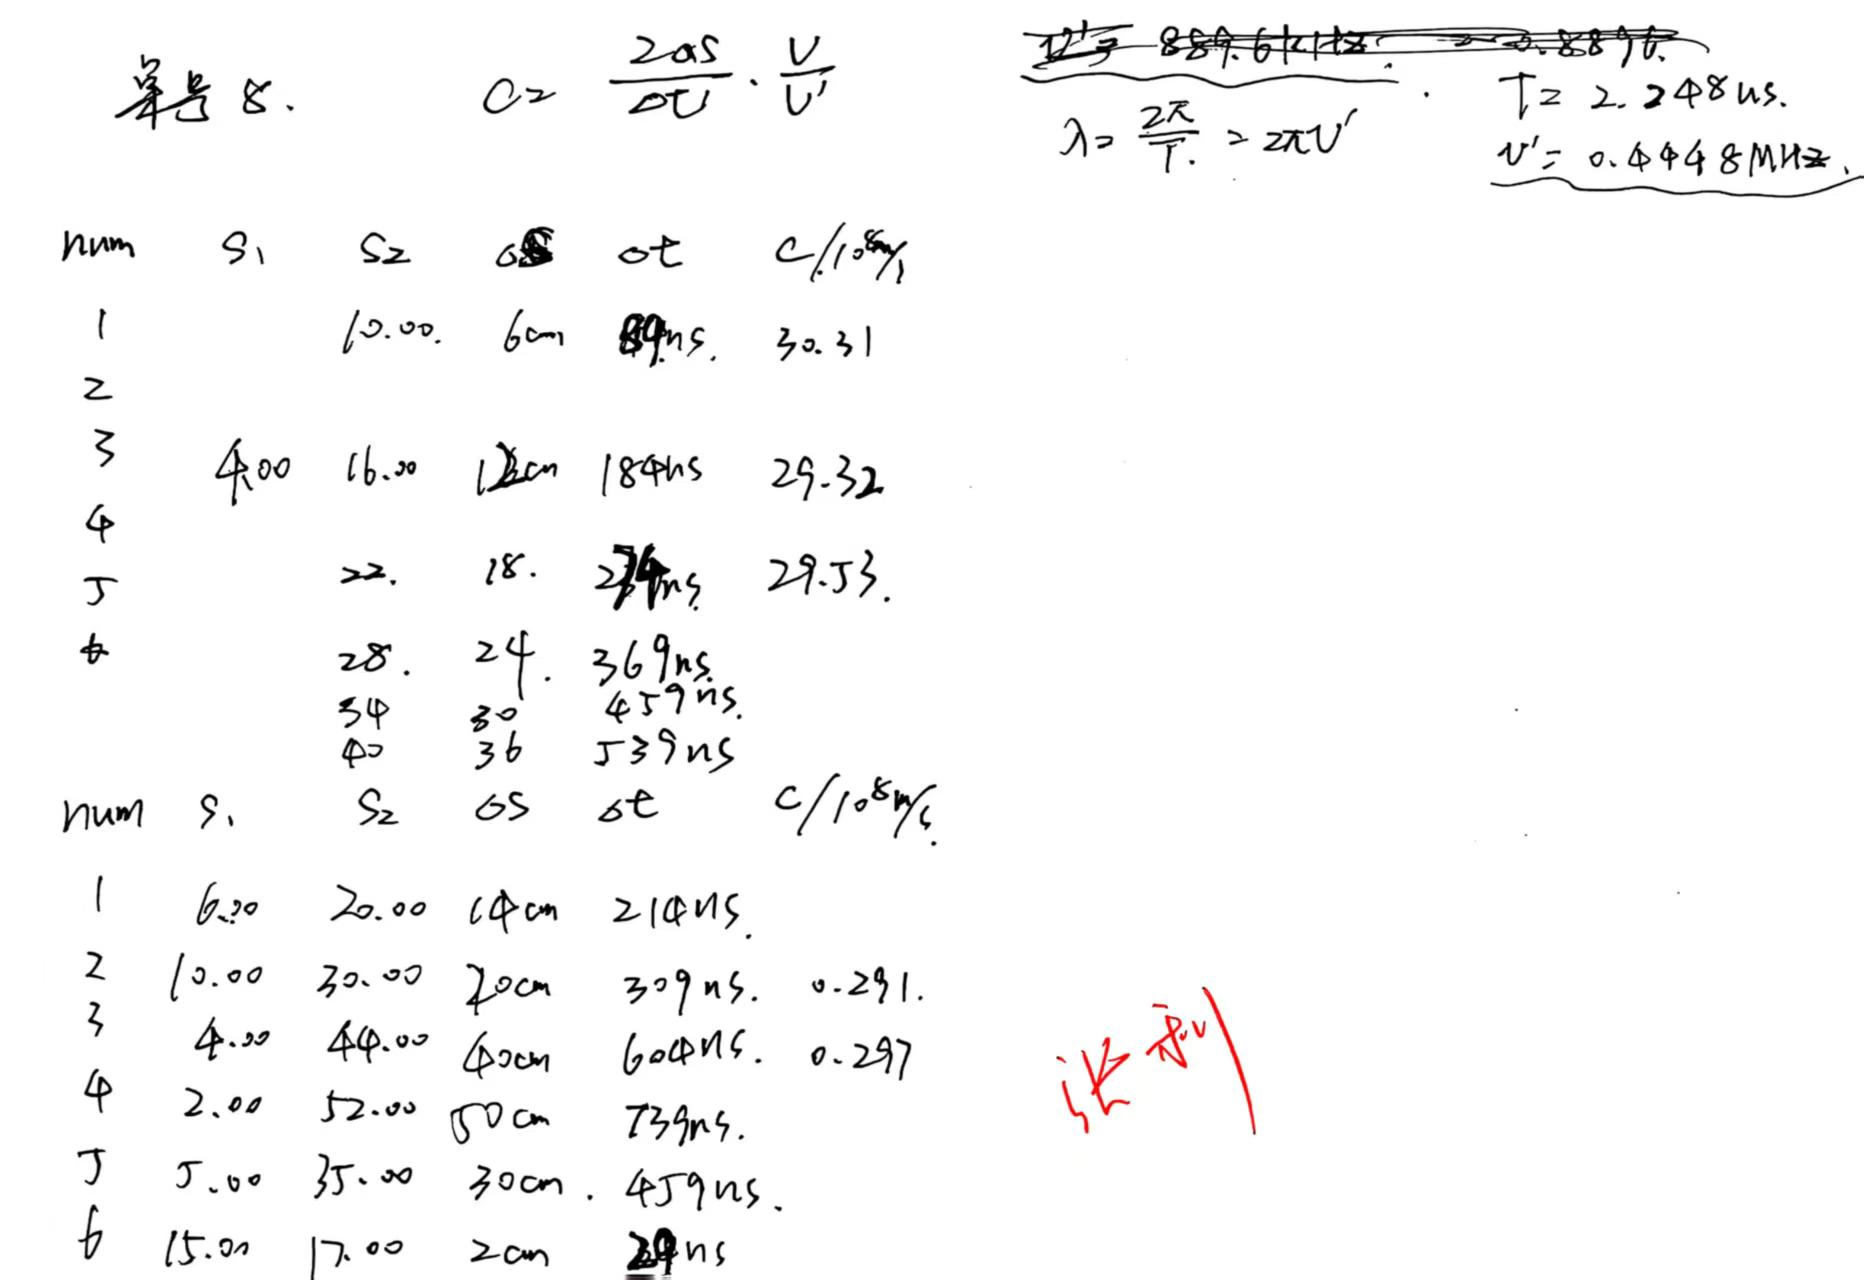
\includegraphics[width=0.55\textwidth]{实验数据原图.jpg}
    \caption{实验数据原图}
    \label{fig:原始数据1}
\end{figure}


\section{结果与分析(60分)}
\subsection{数据处理与结果(30分)}

% 光速测量实验数据表格
% 使用multirow美化s1列
\begin{table}[H]
    \centering
    \caption{光速测量实验数据处理表}
    % 在表格最上方添加频率信息并用线框包围
    \renewcommand{\arraystretch}{1.3}
    \setlength{\tabcolsep}{8pt}
    \begin{tabular}{|c|c|c|c|c|c|}
        \hline
        \multicolumn{6}{|c|}{\textbf{$\upsilon = 100\ \mathrm{MHz}$ \quad $\upsilon' = 0.4448\ \mathrm{MHz}$}} \\
        \hline
        次数 & $s_1$/cm & $s_2$/cm & $\Delta s$/cm & $\Delta t$/ns & $c/(10^8\,\mathrm{m}/\mathrm{s})$ \\
        \hline
        1  & \multirow{6}{*}{4}  & 10 & 6  & 89  & 3.0313 \\
        2  &                      & 16 & 12 & 184 & 2.9324 \\
        3  &                      & 22 & 18 & 274 & 2.9538 \\
        4  &                      & 28 & 24 & 369 & 2.9245 \\
        5  &                      & 34 & 30 & 459 & 2.9388 \\
        6  &                      & 40 & 36 & 539 & 3.0032 \\
        \hline
        7  & 6  & 20 & 14 & 214 & 2.9416 \\
        8  & 10 & 30 & 20 & 309 & 2.9103 \\
        9  & 4  & 44 & 40 & 604 & 2.9778 \\
        10 & 2  & 52 & 50 & 739 & 3.0422 \\
        11 & 5  & 35 & 30 & 459 & 2.9388 \\
        12 & 15 & 17 & 2  & 29  & 3.1010 \\
        \hline
    \end{tabular}
\end{table}

\textbf{接下来我们对实验数据进行简单地处理:}我们将采用三种不同的方法计算光速的估计值。
\subsubsection{平均值法:}计算上述数据的平均值作为光速的估计值。
计算得:
\begin{equation}
    \bar{c} = \frac{1}{12} \sum_{i=1}^{12} c_i = 2.9733 \times 10^8\ \mathrm{m/s}
\end{equation}
\subsubsection{逐差法:}计算相邻两次测量的光程差和时间差,得到更精确的光速估计值。
计算得:
\begin{equation}
    c = \frac{2(\Delta s_2 - \Delta s_1)\upsilon }{(\Delta t_2 - \Delta t_1) \upsilon '} = \frac{2(12 - 6)\ \mathrm{cm} \times 100\ \mathrm{MHz}}{(184 - 89)\ \mathrm{ns} \times 0.4448\ \mathrm{MHz}} = 3.014\times 10^8\ \mathrm{m/s}
\end{equation}

\subsubsection{斜率拟合法:}将光程差 $\Delta s$ 作为横坐标,时间差 $\Delta t$ 作为纵坐标,进行线性拟合,斜率 $k$ 即为 $\frac{\Delta t}{\Delta s}$。
根据公式 $c = 2k \times \frac{\upsilon}{\upsilon'}$ 计算光速。
使用Matlab进行线性拟合,拟合图如下:

\begin{figure}[H]
    \centering
    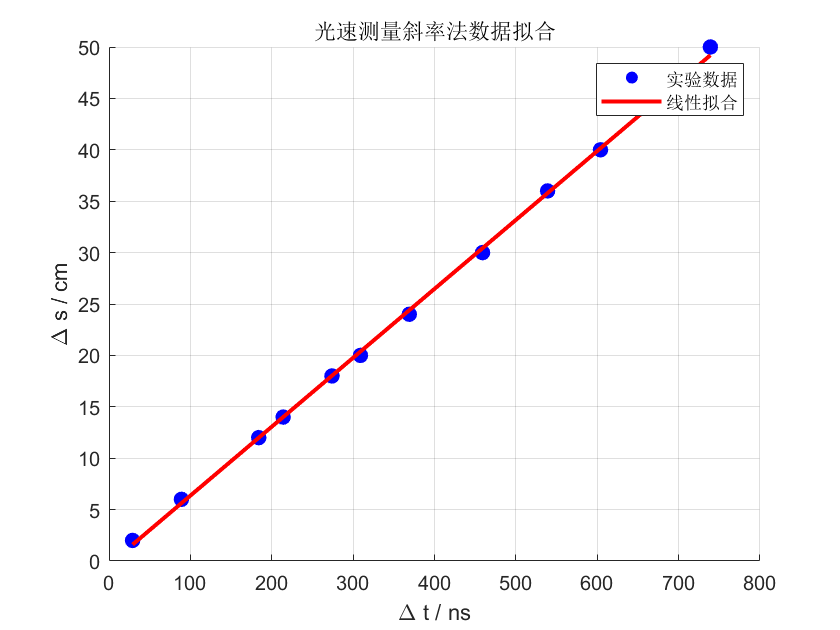
\includegraphics[width=0.6\textwidth]{线性拟合图.png}
    \caption{线性拟合图}
    \label{fig:线性拟合图}
\end{figure}

得到斜率 $k = 0.0670\ \mathrm{cm/ns}$。
计算得:
\begin{equation}
    c = 2k \times \frac{\upsilon}{\upsilon'} = 2 \times 0.0670\ \mathrm{cm/ns} \times \frac{100\ \mathrm{MHz}}{0.4448\ \mathrm{MHz}} = 3.015\times 10^8\ \mathrm{m/s}
\end{equation}

\newpage

\subsection{误差分析(20分)}
本实验的主要误差来源包括仪器读数误差、数据处理方法误差以及环境因素影响。下面分别进行分析:

\textbf{1. 仪器读数误差:}
\begin{itemize}
    \item 距离 $s$ 的测量误差主要来自标尺的最小分度值和人为读数误差。
    \item 时间 $\Delta t$ 的测量误差主要来自示波器的分辨率和光标定位误差。
\end{itemize}

\textbf{2. 数据处理方法误差:}
\begin{itemize}
    \item 采用斜率法和逐差法时,若数据点分布不均或存在系统性偏差,会影响最终结果。
\end{itemize}

\textbf{3. 环境因素:}
\begin{itemize}
    \item 光路调整不理想、反射镜未完全对准、环境光干扰等都会影响信号质量。
\end{itemize}

\textbf{4. A类不确定度分析:}

A类不确定度主要来源于多次独立测量的统计波动。以光速 $c$ 的多次测量值 $c_i$ 为例,A类不确定度按如下公式计算:

\begin{equation}
    u_A = \sqrt{\frac{1}{n(n-1)} \sum_{i=1}^n (c_i - \bar{c})^2}
\end{equation}
其中 $n$ 为测量次数,$c_i$ 为每次测得的光速,$\bar{c}$ 为平均值。

根据实验数据,$n=12$,代入各 $c_i$ 可得:

\begin{equation}
    u_A = \sqrt{\frac{1}{12 \times 11} \sum_{i=1}^{12} (c_i - 2.9733 \times 10^8)^2}
\end{equation}

计算得 $u_A \approx 0.053 \times 10^8\ \mathrm{m/s}$。

因此,最终结果可表示为:

\begin{equation}
    c = (2.97 \pm 0.05) \times 10^8\ \mathrm{m/s}
\end{equation}

最终结果和使用逐差法、斜率拟合法得到的结果也较为吻合,说明数据处理方法合理。

\subsection{实验探讨(10分)}
本实验通过光调制法间接测量光速,利用转化的方法把原来难以测量的光速转化为易于测量的电信号,方法简便操作简单,且具有较高的精度。最终呈现出来的光速值与国际公认值 $c \approx 3.00 \times 10^8\ \mathrm{m/s}$ 非常接近,说明实验设计比较合理。

实验中数据线性关系良好,说明理论模型与实际情况吻合较好。通过多次测量和不同数据处理方法,结果基本相互吻合,进一步验证了实验的可靠性。

本实验综合考虑了多种可能的误差,采用多种数据处理方法,使最后结果的可信度较高。若能进一步减小读数误差,增加更多组数据,结果将更接近理论值。


\newpage
\section{思考题(10分)}
\subsection{思考题1:实验中可能出现波形假位移,如何克服?}

实验中可能出现的波形假位移可能是由于环境内原本光线的干扰造成的,或者是光路没有调节精准,导致接收器接收到的光信号不稳定。
为克服这些问题,可以采取以下措施:

1. 在实验室内尽量减少其他光源的干扰,使用遮光罩或在暗室中进行实验。

2. 在实验前调节光路,确保发射光能准确地反射回接收器中心。

3. 多次测量:通过多次测量取平均值,减小偶然误差的影响。

\subsection{思考题2:分析影响实验精度的主要因素。}

影响实验精度主要有以下几个方面:

1. 光标选取误差。在实验中需要让示波器的AX和BX光标都对应波形的同一点,但是由于调节本身的精度限制和人工调节的误差,难免对$\Delta t$的测量产生影响。

2. 光程差测量误差。光程差的测量依赖人工读数,一些微小的偏差和读数失误都可能导致测量结果的不准确。

3. 环境因素。实验环境中的光线干扰等因素都有可能影响实验结果的精度

\subsection{思考题3:描述光速测量的其他实验方法。}

除了本实验中采用的光调制法测量光速外,还有其他几种有名的光速测量方法:

1. 旋转齿轮法:这是最早的地面光速测量方法之一。通过让光线穿过一个高速旋转的齿轮,光线经过一定距离后反射回来,再次通过齿轮。如果齿轮转速合适,反射回来的光线会被齿轮的齿挡住或通过,从而根据齿轮的转速和光程长度计算出光速。

2. 旋转镜法:该方法改进了旋转齿轮法,采用高速旋转的多面镜代替齿轮。光线经过旋转镜反射后,经过长距离反射回来,再次被旋转镜反射。通过测量旋转镜的转速和光程,可以精确计算光速。该方法大大提高了测量精度。

3. 激光干涉法:利用迈克尔逊干涉仪,通过比较不同路径的光程差,测量干涉条纹的移动,从而精确计算光速。该方法精度极高,常用于现代物理实验室。


\vspace{1cm}
{\fangsong \noindent \textbf{注意事项:}

\begin{enumerate}[label=\arabic*.]
    \item 用PDF格式上传“预习报告”,文件名:学生姓名+学号+实验名称+周次。
    \item “预习报告”必须递交在“学在浙大”本课程内对应实验项目的“作业”模块内。
    \item “预习报告”还须拷贝到“实验报告”中(以便教师批改)。
    \item “大学物理实验”课程选做实验使用本“预习报告”;必做实验无须写预习报告,前往“学在浙大”完成预习测试即可。
\end{enumerate}}
\begin{center}
    \fbfangsong{浙江大学物理实验教学中心制}
\end{center}
\end{document}
